\documentclass[border=3pt,tikz]{standalone}
% Shared look for every TikZ figure in these notes.
% Included by each standalone figure file; also keeps the figures consistent
% with the colours used in the PDF and on the website.

\usepackage{tikz}
\usepackage{pgfplots}
\pgfplotsset{compat=1.18}
\usetikzlibrary{arrows.meta, decorations.markings, decorations.pathmorphing,
                patterns, calc, positioning}
\usepackage{amsmath}

% Series colours are the three validated categorical slots also used by the
% interactive widgets, so a path drawn in the printed notes and the same path on
% the website are the same colour. They clear the colour-vision-deficiency and
% contrast checks as a set; every path is direct-labelled as well, so colour is
% never the only thing carrying identity.
\definecolor{duPurple}{HTML}{68246D}
\definecolor{duBlue}{HTML}{2A78D6}
\definecolor{duRed}{HTML}{EB6834}
\definecolor{duGreen}{HTML}{1BAF7A}
\definecolor{duGrey}{HTML}{4D4D4D}

\tikzset{
  % heavier default lines and arrow tips, so diagrams stay clear when zoomed
  every picture/.append style = {line width=0.7pt, >={Stealth[length=3mm]}},
  axisline/.style   = {-{Stealth[length=3.4mm]}, line width=1.0pt, black},
  path1/.style      = {duBlue,   line width=1.6pt},
  path2/.style      = {duRed,    line width=1.6pt},
  path3/.style      = {duGreen,  line width=1.6pt},
  statedot/.style   = {circle, fill=black, inner sep=1.8pt},
  arrowhead/.style  = {decoration={markings,
                        mark=at position #1 with {\arrow{Stealth[length=3.4mm]}}},
                       postaction={decorate}},
  lbl/.style        = {font=\normalsize},
  slbl/.style       = {font=\small, duGrey},
  workfill/.style   = {duPurple, opacity=0.16},
}

% larger labels in plots as well
\pgfplotsset{every axis/.append style={label style={font=\normalsize}, tick label style={font=\small}, line width=0.9pt}}

% Two blocks, one hot and one cold, brought into contact: heat flows from hot
% to cold until both reach the same temperature (thermal equilibrium).
\begin{document}
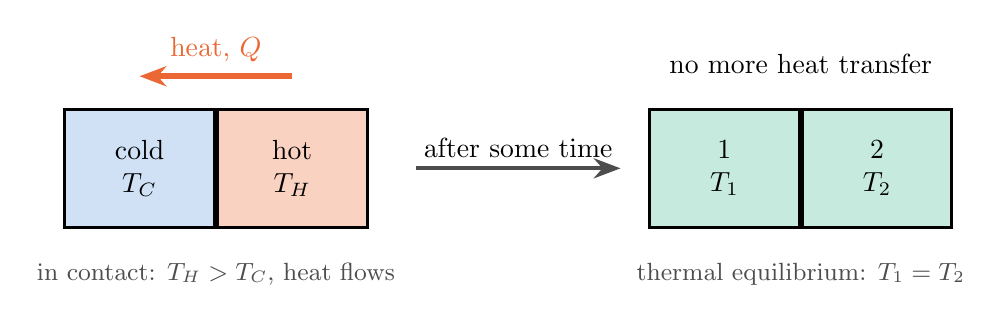
\begin{tikzpicture}[
  blk/.style = {draw, line width=1.1pt, minimum width=19mm, minimum height=15mm,
                font=\normalsize, align=center},
]
% ---- before: hot and cold in contact ------------------------------------
\node[blk, fill=duBlue!22] (c) at (0,0) {cold\\$T_C$};
\node[blk, fill=duRed!30, anchor=west] (h) at (c.east) {hot\\$T_H$};
\draw[-{Stealth[length=3.4mm]}, line width=2pt, duRed]
  ([yshift=4mm]h.north) -- ([yshift=4mm]c.north)
  node[midway, above=1pt, font=\normalsize] {heat, $Q$};
\node[slbl, below=3mm] at (c.south east) {in contact: $T_H > T_C$, heat flows};

% ---- time passes ---------------------------------------------------------
\draw[-{Stealth[length=3.4mm]}, line width=1.4pt, duGrey]
  ([xshift=6mm]h.east) -- ++(2.6,0) node[midway, above, font=\normalsize, black] {after some time};

% ---- after: same temperature ---------------------------------------------
\node[blk, fill=duGreen!25, anchor=west] (a) at ([xshift=35.5mm]h.east) {1\\$T_1$};
\node[blk, fill=duGreen!25, anchor=west] (b) at (a.east) {2\\$T_2$};
\node[font=\normalsize, above=3mm] at (a.north east) {no more heat transfer};
\node[slbl, below=3mm] at (a.south east) {thermal equilibrium: $T_1 = T_2$};
\end{tikzpicture}
\end{document}
